% =============================================================================
% Brazil mental health reform — a DiD checklist walkthrough
% Glasgow workshop, Scott Cunningham
%
% Uses: remix.sty (Glasgow workshop style)
% =============================================================================

\documentclass[aspectratio=169,12pt,t]{beamer}
\usepackage{remix}
\usepackage{booktabs}
\usepackage{array}
\usepackage{ragged2e}
\usepackage{listings}
\usepackage{colortbl}
\usetikzlibrary{arrows.meta, positioning, calc, backgrounds}

\renewcommand{\remixfooter}{The Remix\,\textperiodcentered\,Glasgow\,\textperiodcentered\,May 2026}

% -----------------------------------------------------------------------------
% Listings style for Stata snippets
% -----------------------------------------------------------------------------
\lstdefinelanguage{Stata}{
  morekeywords={reg, regress, gen, generate, replace, by, bysort, drop, keep,
                sort, use, save, clear, set, seed, obs, expand, label, egen,
                sum, summarize, display, capture, log, close, exit, if, in,
                ssc, install, csdid, csdid2, drdid, ivar, time, gvar, ipw,
                dripw, drimp, long2, notyet, wboot, reps, panelview, honestdid,
                preserve, restore, foreach, forvalues, local, global, matrix,
                xtset, probit, predict, twoway, histogram, scatter, graph,
                contract, file, write, open},
  sensitive=true,
  morecomment=[l]{*},
  morecomment=[l]{//},
  morestring=[b]",
}
\lstset{
  basicstyle=\ttfamily\footnotesize,
  keywordstyle=\color{remixgreendark}\bfseries,
  commentstyle=\color{warmgray}\itshape,
  stringstyle=\color{ocean},
  backgroundcolor=\color{lightbg},
  frame=single,
  framesep=4pt,
  rulecolor=\color{warmgray!40},
  columns=fullflexible,
  showstringspaces=false,
  breaklines=true,
  numbers=none,
  xleftmargin=0.4em,
  xrightmargin=0.4em,
}

% Suppress harmless box warnings
\AtBeginDocument{\hfuzz=45pt\vfuzz=30pt}

% =============================================================================
\begin{document}
% =============================================================================

% ----------------------------------------------------------------------------
% TITLE
% ----------------------------------------------------------------------------
\remixtitleframe
  {A DiD Checklist}
  {Walking through the Brazil mental health reform, step by step}
  {Scott Cunningham \textperiodcentered\ Baylor University}
  {Glasgow \textperiodcentered\ May 2026}

% =============================================================================
% PART I — The paper
% =============================================================================

% ----------------------------------------------------------------------------
% Slide 2: The paper
% ----------------------------------------------------------------------------
\begin{frame}{Today's example: the Brazil mental health reform}
\vspace{0.5cm}

\textbf{Dias \& Fontes (2024)} \\
\textit{``The Effects of a Large-Scale Mental Health Reform: Evidence from Brazil''} \\
\textit{American Economic Journal: Economic Policy}, 16(3): 257--289

\vspace{0.7cm}

\textbf{What they study.} \;Brazil's 2002 psychiatric reform replaced large inpatient hospitals with \textit{community mental health centers} (CAPS) --- a major deinstitutionalization push.

\vspace{0.4cm}

\highlight{Why we use it here.} \;It is a clean staggered rollout, with a large panel of municipalities, and the right ingredients for a real DiD checklist.
\end{frame}

% ----------------------------------------------------------------------------
% Slide 3: The reform
% ----------------------------------------------------------------------------
\begin{frame}{The reform in one slide}
\vspace{0.5cm}

\textbf{What CAPS is.} \;A \textit{Centro de Aten\c{c}\~ao Psicossocial} --- a community mental health center providing outpatient care, day programs, and psychosocial support. \;The reform created CAPS centers as a substitute for inpatient psychiatric hospitals.

\vspace{0.5cm}

\textbf{Scale.} \;Over 1{,}600 CAPS centers opened across 5{,}180 municipalities between 2002 and 2016. \;A municipality is either treated (gets a CAPS in some year) or never treated.

\vspace{0.5cm}

\highlight{This is the canonical setup for staggered DiD:} \;many units, different treatment dates, a long enough panel to see pre- and post-trends.
\end{frame}

% ----------------------------------------------------------------------------
% Slide 4: The headline finding
% ----------------------------------------------------------------------------
\begin{frame}{The headline finding}
\vspace{0.3cm}

\textbf{What worked.}
\begin{itemize}\small\setlength\itemsep{0pt}
  \item Increased \textbf{outpatient mental health care} use.
  \item \textbf{Reduced psychiatric hospitalizations}.
\end{itemize}

\vspace{0.3cm}

\textbf{What didn't.}
\begin{itemize}\small\setlength\itemsep{0pt}
  \item \textit{\textbf{Increased homicide rates}} --- deinstitutionalization channel: vulnerable patients in the community without supervision.
  \item Hospital savings did not offset the social cost.
\end{itemize}

\vspace{0.2cm}
\meta{We'll focus on the homicide-rate outcome.}
\end{frame}

% =============================================================================
% PART II — The checklist
% =============================================================================

% ----------------------------------------------------------------------------
% Slide 5: Why a checklist
% ----------------------------------------------------------------------------
\begin{frame}{A checklist for staggered DiD}
\vspace{0.3cm}

\textit{The Checklist Manifesto} (Gawande, 2009) makes the case that even highly skilled experts skip steps under cognitive load. \;Pilots, surgeons, structural engineers --- all use written checklists. \;Empiricists should too.

\vspace{0.4cm}

\textbf{For staggered DiD, the steps are:}
\vspace{0.1cm}
\begin{columns}[T,onlytextwidth]
\column{0.48\textwidth}
\begin{enumerate}\small\setlength\itemsep{1pt}
  \item Define the target parameter.
  \item Tabulate when units are treated.
  \item Plot the rollout.
  \item Plot the outcome by cohort.
  \item Select covariates --- with discipline.
\end{enumerate}
\column{0.48\textwidth}
\begin{enumerate}\small\setlength\itemsep{1pt}\setcounter{enumi}{5}
  \item Inspect the propensity score.
  \item Estimate (CS, BJS, $\ldots$).
  \item Run an event study (universal baseline).
  \item Sensitivity analysis (Rambachan--Roth).
\end{enumerate}
\end{columns}
\end{frame}

% =============================================================================
% STEP 1 — Define the target parameter
% =============================================================================

% ----------------------------------------------------------------------------
% Slide 6: Step 1 setup
% ----------------------------------------------------------------------------
\begin{frame}{Step 1: Define the target parameter}
\vspace{0.6cm}

\textbf{What is the question?} \;Did opening a CAPS center, in the years after it opened, change the homicide rate in that municipality?

\vspace{0.5cm}

\textbf{Three ingredients} go into any target parameter:
\vspace{0.3cm}
\begin{enumerate}\setlength\itemsep{4pt}
  \item A \textit{difference in potential outcomes} \;$Y(1) - Y(0)$.
  \item A \textit{population} on which we average it.
  \item A \textit{weighting} rule \;$\mathbb{E}[\,\cdot\,]$.
\end{enumerate}

\vspace{0.5em}
\meta{Most disagreements about ``the'' DiD estimand are disagreements about which of these three you chose.}
\end{frame}

% ----------------------------------------------------------------------------
% Slide 7: ATT
% ----------------------------------------------------------------------------
\begin{frame}{The target: ATT on the treated, in post-treatment periods}
\vspace{0.3cm}

\[
\text{ATT} \;=\; \mathbb{E}\Big[\;\underbrace{Y_{it}(1) - Y_{it}(0)}_{\text{(1) PO contrast}}\;\Big|\;\underbrace{D_i = 1,\;\text{Post}_t}_{\text{(2) population}}\;\Big]
\]

\vspace{0.35cm}

\textbf{In our case:}
\begin{itemize}\small\setlength\itemsep{0pt}
  \item \textbf{Contrast.} \;Y(1) = homicide rate with a CAPS; Y(0) = homicide rate without one.
  \item \textbf{Population.} \;Municipalities that \textit{actually got} a CAPS, after they got it.
  \item \textbf{Weighting.} \;Group-time ATTs ($g,t$); we'll aggregate later.
\end{itemize}

\vspace{0.3em}
\highlight{Decide this \textit{first}.} \;Every downstream choice is meant to identify \textit{this} parameter.
\end{frame}

% =============================================================================
% STEP 2 — Cohort table
% =============================================================================

% ----------------------------------------------------------------------------
% Slide 8: Step 2 setup
% ----------------------------------------------------------------------------
\begin{frame}{Step 2: Tabulate when units are treated}
\vspace{0.6cm}

Before anything else, count the cohorts: \;how many municipalities got a CAPS in each year, and how many were never treated.

\vspace{0.5cm}

\textbf{Why this table earns its place on the slide.}
\begin{itemize}\small
  \item It defines the \textbf{groups} ($g$) in the estimator.
  \item It tells you which cohort is the \textit{smallest} --- which sets a binding constraint on covariate count (see Step 5).
  \item It tells you which units are \textit{always treated} (must be dropped) and \textit{never treated} (the control group).
\end{itemize}

\vspace{0.4em}
\meta{Next slide: the table itself.}
\end{frame}

% ----------------------------------------------------------------------------
% Slide 9: The cohort table
% ----------------------------------------------------------------------------
\begin{frame}{CAPS introduction by cohort, 2003--2016}
\vspace{-0.05cm}
\begin{center}
\scriptsize
\setlength{\tabcolsep}{5pt}
\renewcommand{\arraystretch}{0.85}
\begin{tabular}{lrrr}
\toprule
\textbf{Cohort} & \textbf{Municipalities} & \textbf{Share of treated} & \textbf{Max cov.\ (EPV $\leq$ 7)} \\
\midrule
\rowcolor{remixgreenlight!50} 2003 & 47   & 3.5\%  & \textbf{6} \;(binds) \\
2004 & 70   & 5.2\%  & 10 \\
2005 & 95   & 7.1\%  & 13 \\
\rowcolor{remixgreenlight!50} 2006 & \textbf{216}  & \textbf{16.1\%} & 30 \;(largest) \\
2007 & 105  & 7.8\%  & 15 \\
2008 & 112  & 8.3\%  & 16 \\
2009 & 75   & 5.6\%  & 10 \\
2010 & 96   & 7.1\%  & 13 \\
2011 & 79   & 5.9\%  & 11 \\
2012 & 114  & 8.5\%  & 16 \\
2013 & 80   & 6.0\%  & 11 \\
2014 & 97   & 7.2\%  & 13 \\
2015 & 80   & 6.0\%  & 11 \\
2016 & 78   & 5.8\%  & 11 \\
\midrule
\textbf{Treated total} & \textbf{1{,}344} & \textbf{100\%} & --- \\
Always-treated (2002, excluded) & 296 & --- & --- \\
Never-treated controls & 3{,}836 & --- & --- \\
\bottomrule
\end{tabular}
\end{center}
\vspace{0.05cm}
\begin{center}
\meta{2003 binds covariate count; 2006 dominates the simple-aggregation weight.}
\end{center}
\end{frame}

% =============================================================================
% STEP 3 — Plot the rollout
% =============================================================================

\begin{frame}{Step 3: Plot the rollout}
\vspace{0.4cm}

Before any estimator, look at \textit{when} treatment turns on, unit by unit.

\vspace{0.4cm}

\textbf{Why look at it.} \;The rollout picture tells you whether the staggering is rich enough to support staggered DiD (some units treated, some not, treatment dates spread across years), or whether you have a near-event-study problem (most units treated in one or two years).

\vspace{0.3cm}

\meta{Tool: \texttt{panelview} (Yiqing Xu, Stanford). \;Rows are municipalities, columns are years, color encodes pre vs post treatment.}
\end{frame}

\begin{frame}{Brazil CAPS rollout: 5{,}476 municipalities, 2002--2016}
\begin{center}
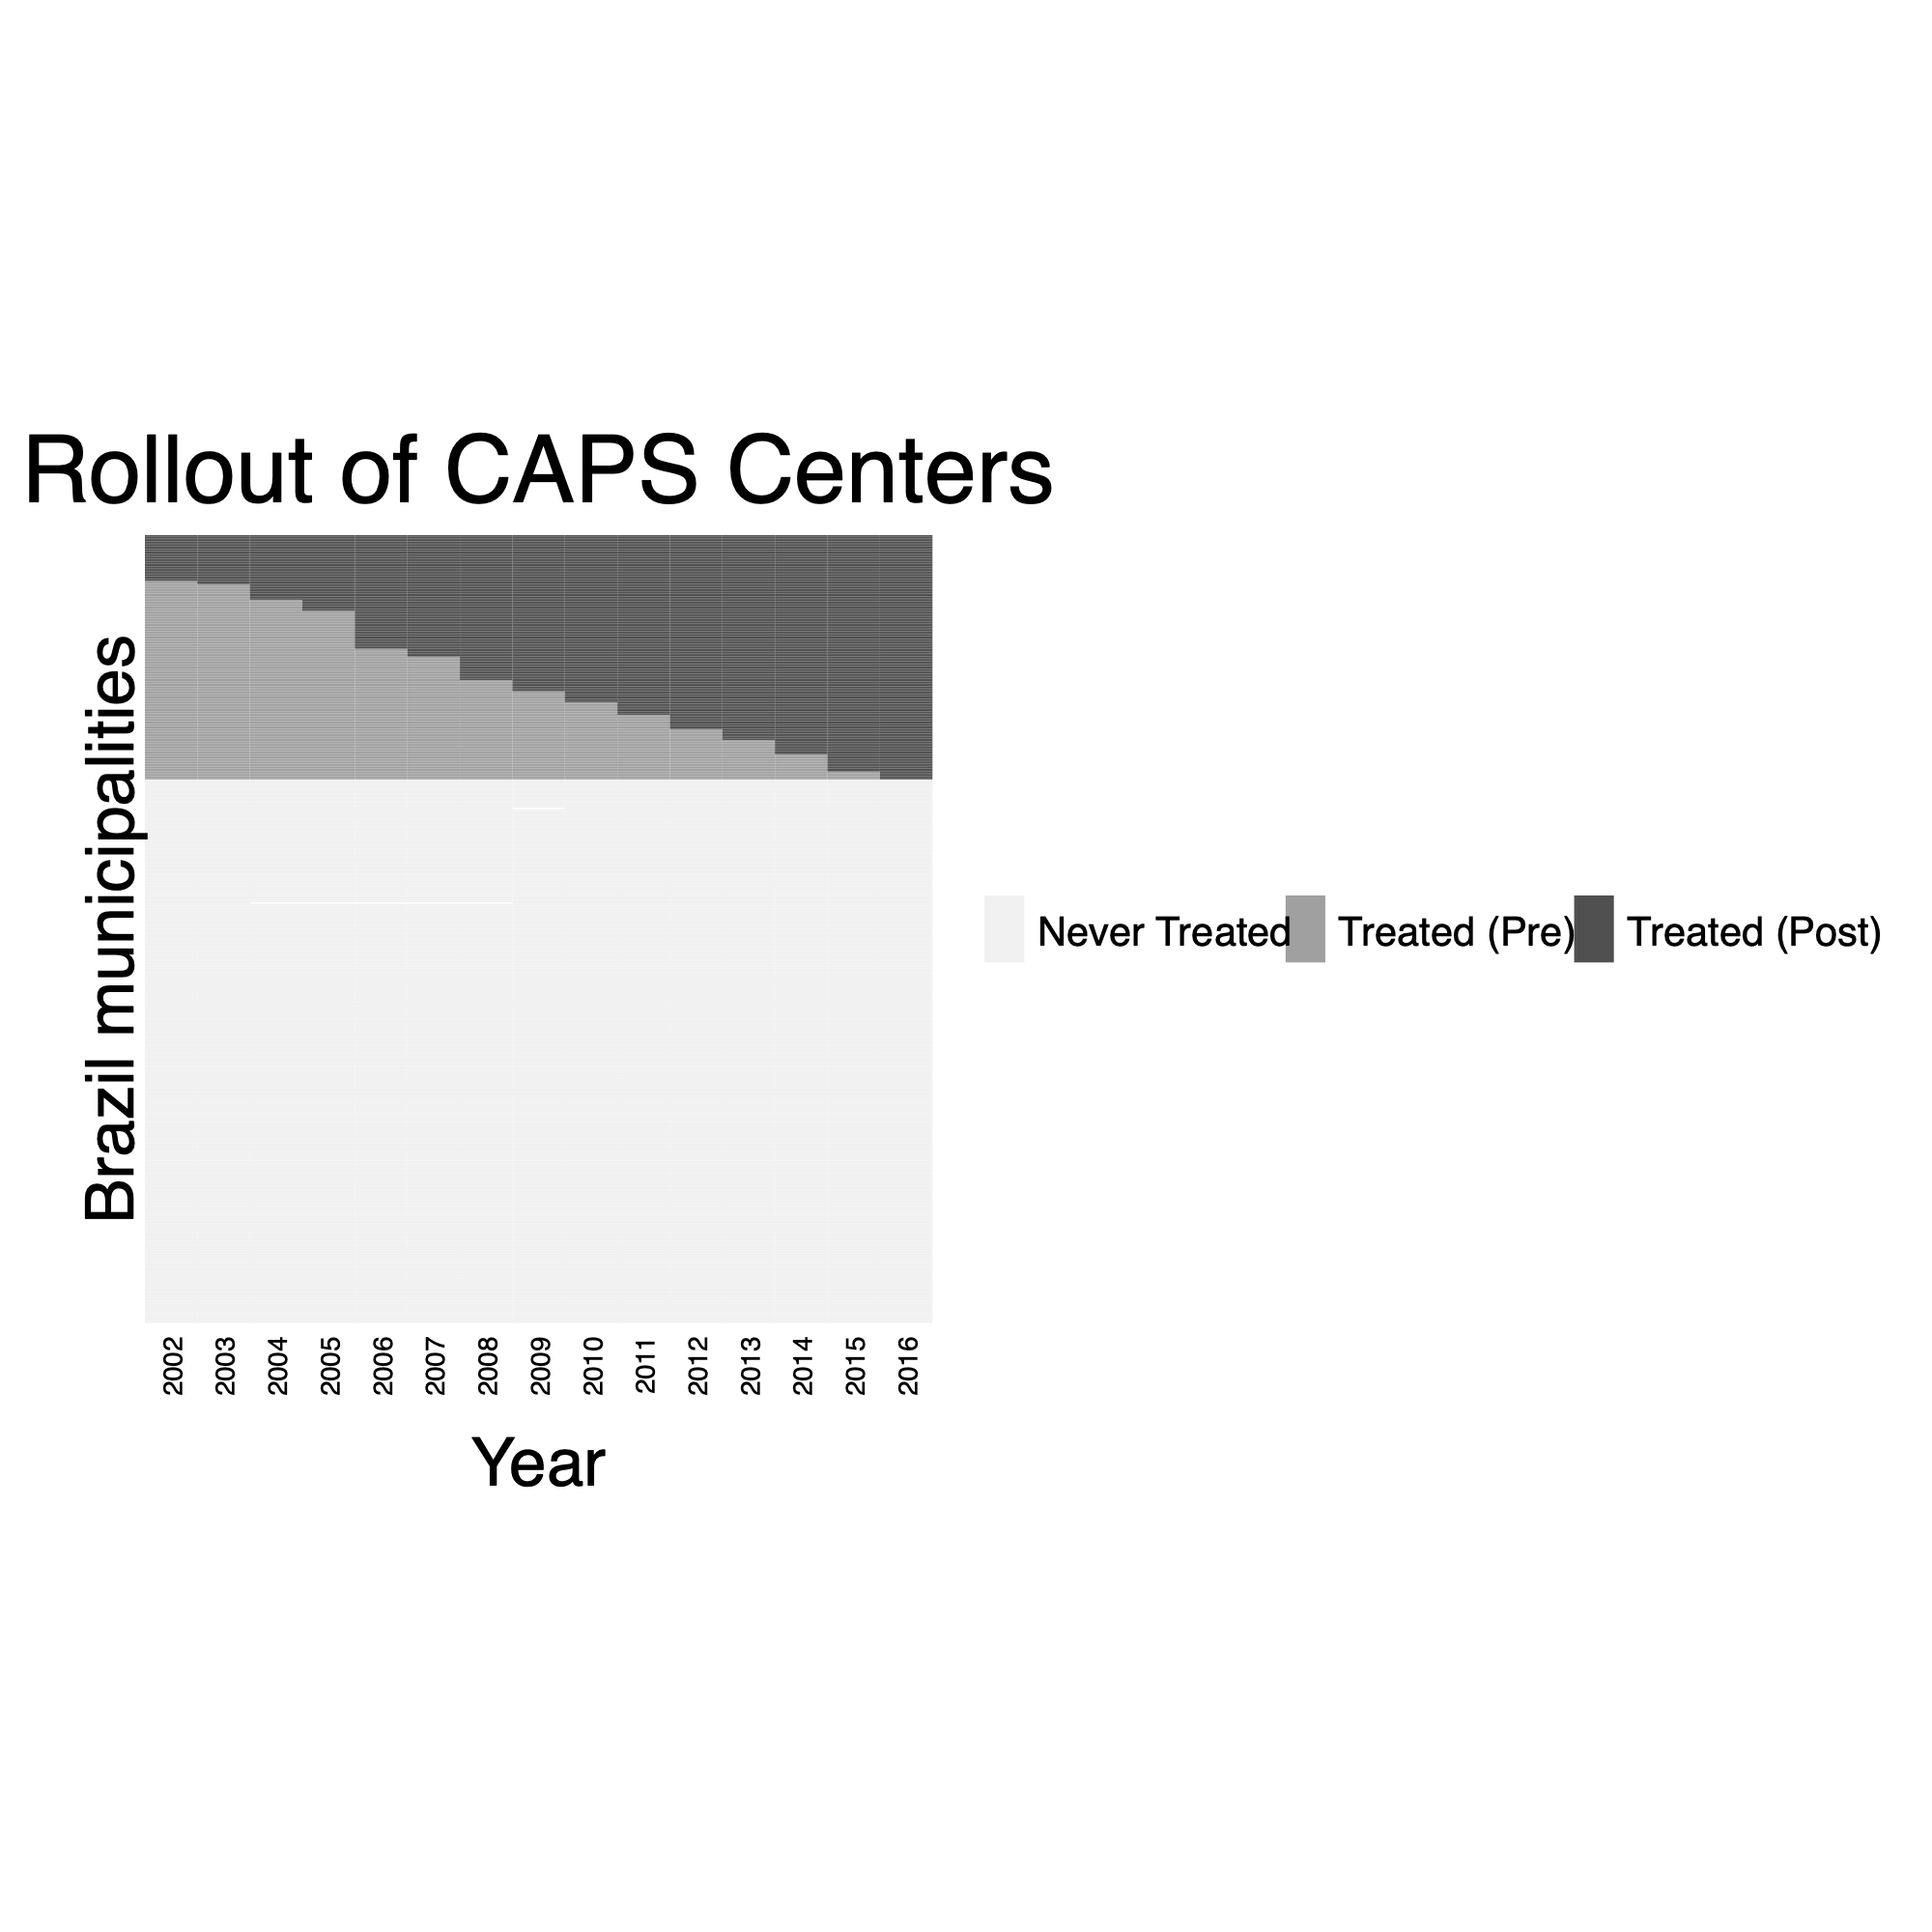
\includegraphics[height=0.72\textheight]{figures/brazil_rollout.png}
\end{center}
\begin{center}
\footnotesize\color{warmgray}\itshape
Light gray = never-treated. \;Medium gray = treated, pre-period. \;Dark gray = treated, post-period.
\end{center}
\end{frame}

% =============================================================================
% STEP 4 — Plot the outcome by cohort
% =============================================================================

\begin{frame}{Step 4: Plot the outcome by cohort}
\vspace{0.4cm}

Now plot the \textit{homicide rate} over time, separately for each cohort. \;Two purposes:

\vspace{0.4cm}
\begin{itemize}\setlength\itemsep{4pt}
  \item See whether trends move in parallel across cohorts in the pre-period.
  \item Catch any anomaly --- a missing year, a level break, an outlier cohort --- before the estimator hides it from you.
\end{itemize}

\vspace{0.5cm}

\highlight{One important reminder.} \;DiD identifies $Y(0)$'s \textit{trend}, not its \textit{level}. \;Levels are differenced away. \;You are looking for parallel \textit{movement}, not for cohorts that overlay each other.

\vspace{0.4em}
\meta{This is the difference between DiD and synthetic control. \;Synth requires comparable levels and trends; \;DiD only needs comparable trends.}
\end{frame}

\begin{frame}{Homicide rate by treatment cohort}
\begin{center}
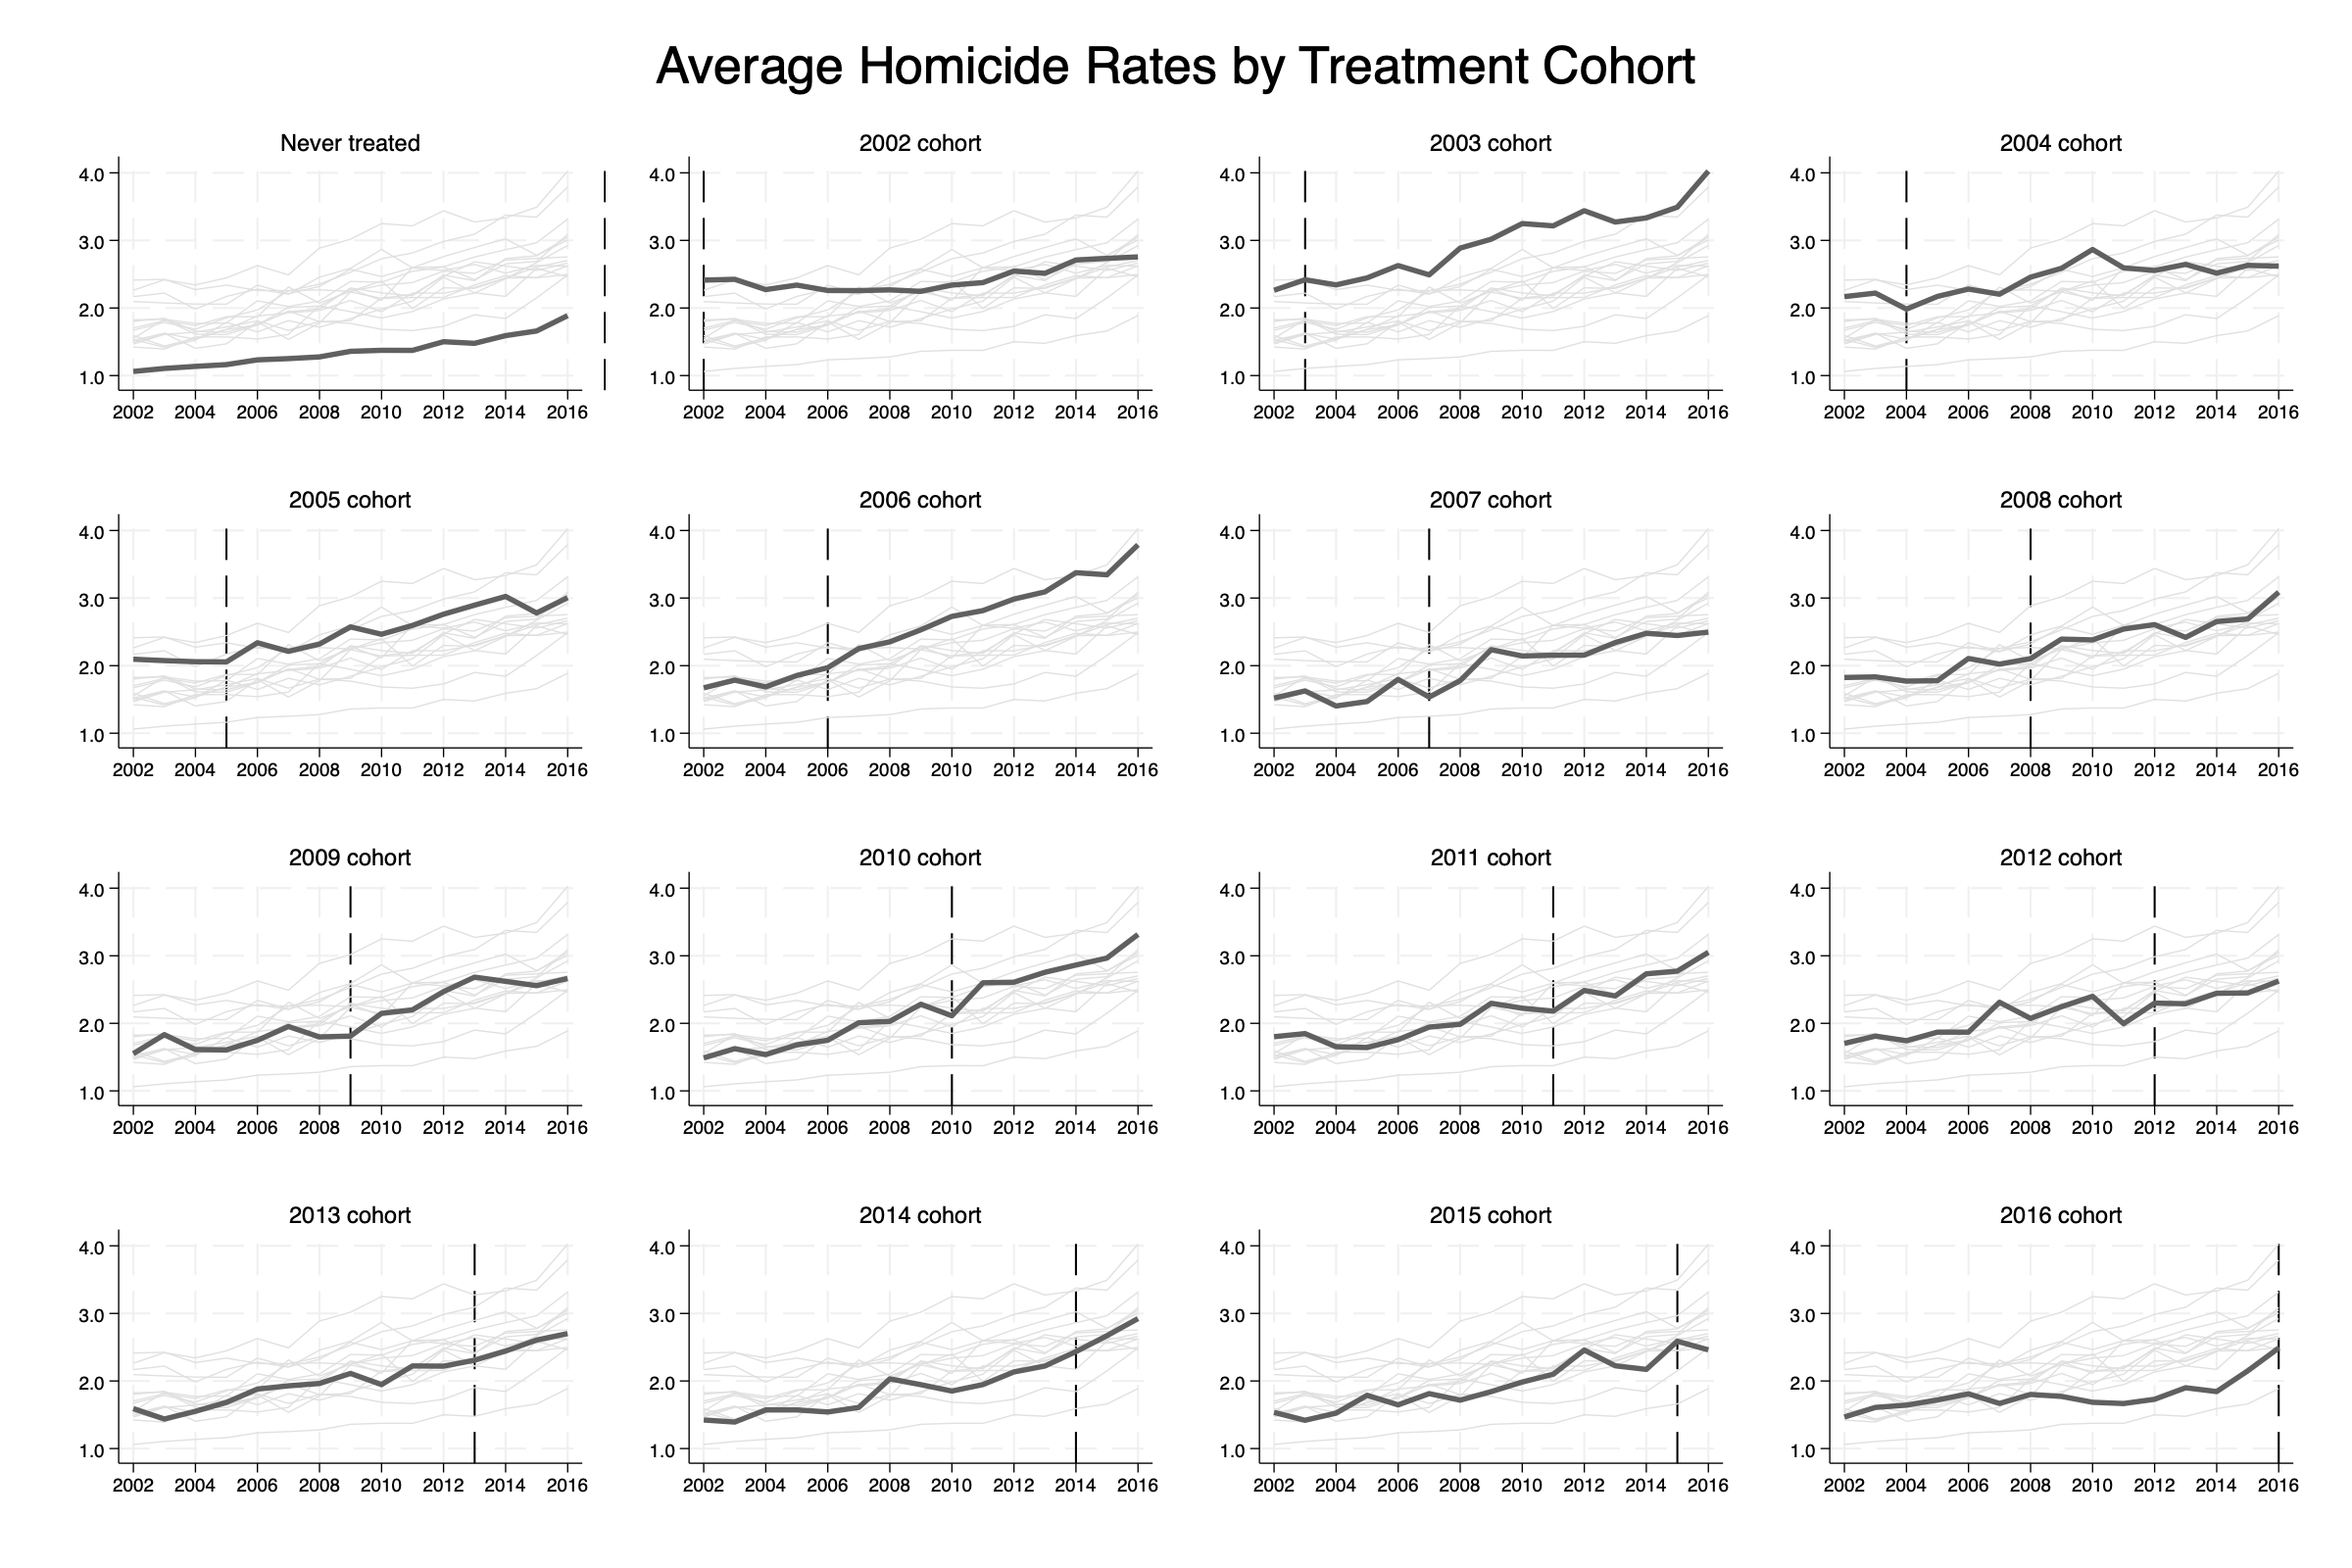
\includegraphics[height=0.72\textheight]{figures/brazil_homicide_by_cohort.png}
\end{center}
\begin{center}
\footnotesize\color{warmgray}\itshape
One small-multiples panel per cohort. \;Bold dark line = focal cohort. \;Dashed vertical = treatment year.
\end{center}
\end{frame}

% =============================================================================
% STEP 5 — Covariate selection
% =============================================================================

\begin{frame}{Step 5: Two ways to think about covariates}
\vspace{0.4cm}

\textbf{Path 1 --- Outcome Regression (OR).} \;Pick covariates that predict $Y(0)$'s \textit{trend}. \;Ask: what are the ordinary drivers of homicide trends in Brazilian municipalities? \;Income, demographics, poverty, urbanization, federal transfers, education.

\vspace{0.5cm}

\textbf{Path 2 --- Propensity Score (PS).} \;Pick covariates that predict \textit{treatment timing}. \;Ask: who got a CAPS first? \;Larger cities? \;Poorer states? \;Earlier hospital capacity?

\vspace{0.5cm}

\highlight{Doubly robust uses both.} \;If you can correctly specify either the outcome trend or the propensity score, DR is consistent. \;You don't have to be right twice.

\vspace{0.4em}
\meta{Use common sense first. \;Run LASSO or stepwise selection only after a domain-informed shortlist.}
\end{frame}

\begin{frame}{Step 5 (cont.): the 7-events-per-covariate rule}
\vspace{0.4cm}

\textbf{Peduzzi, Concato, Kemper, Holford \& Feinstein (1996),} \;\textit{``A simulation study of the number of events per variable in logistic regression analysis,''} \;\textit{Journal of Clinical Epidemiology}, 49(12): 1373--1379.

\vspace{0.4cm}

\textbf{The rule.} \;A logistic regression needs roughly 7--10 ``events'' (the smaller of the two outcome classes) per covariate to avoid overfit and unstable coefficients.

\vspace{0.4cm}

\textbf{In a propensity score model for staggered DiD,} the ``event'' is the number of treated units in a 2$\times$2 comparison. \;If cohort $g$ has 47 municipalities (our 2003 cohort), the EPV ceiling is roughly $\lfloor 47/7 \rfloor = 6$ covariates.

\vspace{0.4em}
\highlight{Different 2$\times$2's can carry different covariate counts. \;The smallest cohort sets the binding limit.}
\end{frame}

\begin{frame}{Step 5 (cont.): standardize, for the computer's sake}
\vspace{0.5cm}

\textbf{The problem.} \;Some covariates look like \texttt{poptotaltrend = population $\times$ year}. \;In Brazil that can be 150 million or larger. \;When the propensity-score logit tries to invert a matrix with entries that big, it doesn't fail like a textbook tells you --- it fails like a computer.

\vspace{0.5cm}

\textbf{The fix.} \;Convert every continuous covariate to a \textit{z-score}: subtract the mean, divide by the SD. \;Now everything is on the same scale, the matrix inverts cleanly, and your estimates don't shift just because someone changed units.

\vspace{0.5cm}

\highlight{This is not econometrics. \;It is numerical hygiene.} \;The model is the same; only the computer's life is easier.
\end{frame}

\begin{frame}{Step 5 (cont.): the balance table the paper actually used}
\vspace{0.25cm}

The published spec used \textbf{31 covariates} in the propensity score and outcome model. \;The balance table (baseline year 2002, excluding the always-treated 2002 cohort) reports a normalized difference for each one.

\vspace{0.35cm}

\begin{columns}[T,onlytextwidth]
\column{0.48\textwidth}
\textbf{31 candidates included things like}
\begin{itemize}\scriptsize\setlength\itemsep{0pt}
  \item Log GDP per capita
  \item Federal cash-transfer receipts
  \item 14 age $\times$ sex population bins
  \item Rural population share
  \item Pre-period homicide trend
  \item Pre-period health-spending trend
\end{itemize}

\column{0.48\textwidth}
\textbf{Imbalance is real.}
\begin{itemize}\scriptsize\setlength\itemsep{0pt}
  \item \;9 covariates with $|$norm.\ diff.$|$ $>$ 0.25
  \item Largest: \;\texttt{poptotaltrend} \;at \;$+0.69$
  \item Smallest cohort (2003): EPV cap of 6
  \item Largest cohort (2006): EPV cap of 30
\end{itemize}
\end{columns}

\vspace{0.25cm}
\highlight{31 candidates, 6 slots in the binding 2$\times$2.} \;Step 5 picks which 6.
\end{frame}

% =============================================================================
% STEP 6 — Propensity score
% =============================================================================

\begin{frame}{Step 6: Inspect the propensity score}
\vspace{0.4cm}

After picking covariates, fit \texttt{probit treat \$controls if ano==2002} and plot $\widehat{p}(X)$ for treated and untreated municipalities.

\vspace{0.3cm}

\textbf{What you want to see:} \;substantial \textbf{overlap}. \;Treated and untreated propensity-score distributions should share most of their support. \;Mass at $\widehat{p} \approx 1$ for controls is a red flag --- those are units the model thinks should have been treated but weren't.

\vspace{0.3cm}

\textbf{Standard practice:} \;trim controls with $\widehat{p} > 0.995$ before estimating. \;The \texttt{did} R package does this automatically.

\vspace{0.4em}
\meta{Next slide: \;histogram from a fitted PS in our setup.}
\end{frame}

\begin{frame}{Propensity score distribution, by treatment status}
\begin{center}
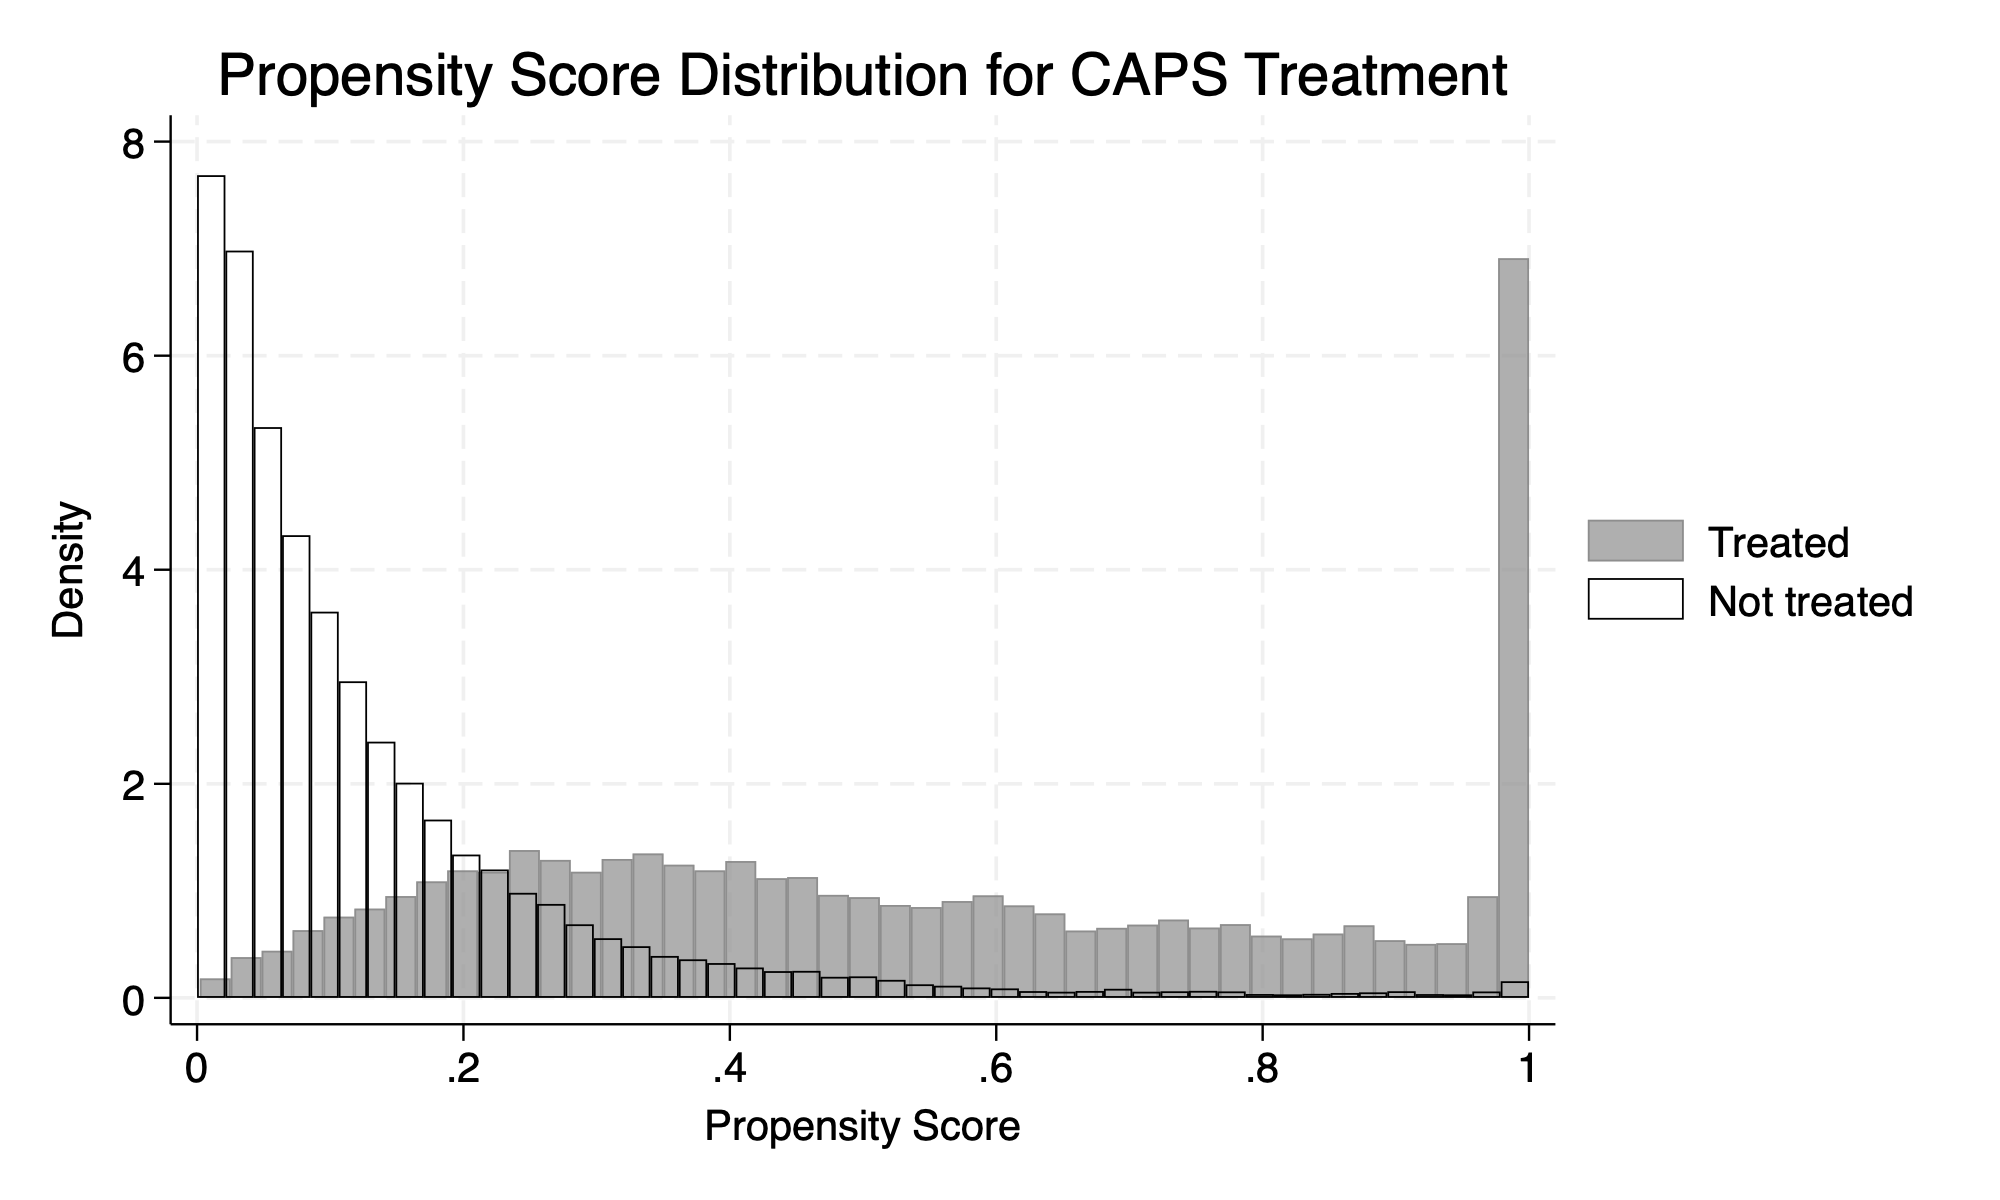
\includegraphics[height=0.72\textheight]{figures/brazil_pscore.png}
\end{center}
\begin{center}
\footnotesize\color{warmgray}\itshape
Gray = treated. \;Black outline = never-treated. \;Mass in the right tail of controls is the trimming target.
\end{center}
\end{frame}

% =============================================================================
% STEP 7 — Estimate with CS
% =============================================================================

\begin{frame}{Step 7: Estimate with the Callaway--Sant'Anna estimator}
\vspace{0.4cm}

Three choices, made deliberately:
\vspace{0.3cm}

\begin{itemize}\setlength\itemsep{4pt}
  \item \textbf{Baseline period.} \;Use \texttt{long2} in Stata / \texttt{base\_period = "universal"} in R. \;This pins every event-time effect to $t = -1$, so pre-trend coefficients are real falsification tests.
  \item \textbf{Estimation method.} \;\texttt{dr} (doubly robust) or \texttt{ipw} or \texttt{reg}. \;DR if you trust neither model individually; OR if you don't want to extrapolate from a logistic regression with overlap problems.
  \item \textbf{Control group.} \;\texttt{notyet} --- not-yet-treated comparison. \;Bigger sample than never-treated only; no pre-trend restriction.
\end{itemize}
\end{frame}

\begin{frame}{Step 7 (cont.): the aggregation question}
\vspace{0.4cm}

\texttt{csdid} returns group-time ATTs: \;$\widehat{\text{ATT}}(g, t)$ for every cohort $g$ and post-period $t$. \;Aggregating these is a choice with consequences.

\vspace{0.5cm}

\begin{itemize}\setlength\itemsep{4pt}
  \item \textbf{Simple ATT.} \;Average over all $(g,t)$ post-treatment cells, weighted by cohort size $\times$ exposure length.
  \item \textbf{Group ATT.} \;First average within cohort to one number per $g$; then average across cohorts.
  \item \textbf{Event-study ATT.} \;Average across cohorts at each event time $e = t - g$.
\end{itemize}

\vspace{0.3em}
\highlight{Big cohorts have big weights.} \;The 2006 cohort (216 units, 16\% of treated) will dominate any size-weighted average.
\end{frame}

\begin{frame}{Step 7 (cont.): a small artifact, to make weighting concrete}
\vspace{0.1cm}

Two cohorts. \;\textbf{Group A}: 5 post-period cells, 500 units each. \;\textbf{Group B}: 2 post-period cells, 100 units each.

\vspace{0.2cm}
\begin{center}
\scriptsize
\setlength{\tabcolsep}{8pt}
\renewcommand{\arraystretch}{1.05}
\begin{tabular}{l|ccccc|cc}
\toprule
                  & \multicolumn{5}{c|}{\textbf{Group A (n = 500)}} & \multicolumn{2}{c}{\textbf{Group B (n = 100)}} \\
cell        & $A_1$ & $A_2$ & $A_3$ & $A_4$ & $A_5$              & $B_1$ & $B_2$ \\
\midrule
$\widehat{ATT}$   & 0.10 & 0.12 & 0.14 & 0.11 & 0.13                 & 0.50 & 0.60 \\
\bottomrule
\end{tabular}
\end{center}

\vspace{0.2cm}
\textbf{Both aggregations weight by population --- just at different units:}
\begin{itemize}\small\setlength\itemsep{0pt}
  \item \textbf{Simple} (each \textit{cell} weighted by $N_g$): \;$\frac{5\cdot 500 \cdot 0.12 \;+\; 2 \cdot 100 \cdot 0.55}{5(500) + 2(100)} = \frac{300 + 110}{2700} = \textbf{0.152}$
  \item \textbf{Group} (each \textit{cohort} weighted by $N_g$): \;$\frac{500\cdot 0.12 \;+\; 100\cdot 0.55}{600} = \frac{60 + 55}{600} = \textbf{0.192}$
\end{itemize}

\vspace{0.05em}
\highlight{Simple amplifies long-exposure cohorts; group neutralizes exposure length.}
\end{frame}

% =============================================================================
% STEP 8 — Event study
% =============================================================================

\begin{frame}{Step 8: The event study, with a universal baseline}
\vspace{0.4cm}

The event study reports $\widehat{\text{ATT}}(e)$ for each event time $e = t - g$. \;Two reasons we use a \textit{universal} baseline ($t = -1$ pinned to zero):

\vspace{0.4cm}

\begin{itemize}\setlength\itemsep{4pt}
  \item \textbf{Pre-trend coefficients become falsification tests.} \;Each pre-period $e < 0$ is now a ``long difference'' relative to $t = -1$. \;The identifying assumption is that \textit{post-period} long differences in $Y(0)$ are zero; pre-period ones should be too.
  \item \textbf{Post-period coefficients become interpretable on the same scale.} \;Every $\widehat{\text{ATT}}(e)$ for $e \geq 0$ is the effect of an additional $e+1$ years of treatment exposure relative to the year before.
\end{itemize}

\vspace{0.4em}
\meta{In Stata: \;\texttt{csdid \ldots\ long2}. \;In R: \;\texttt{base\_period = "universal"} inside \texttt{att\_gt()}.}
\end{frame}

\begin{frame}{The event study: CAPS effect on homicide rates}
\begin{center}
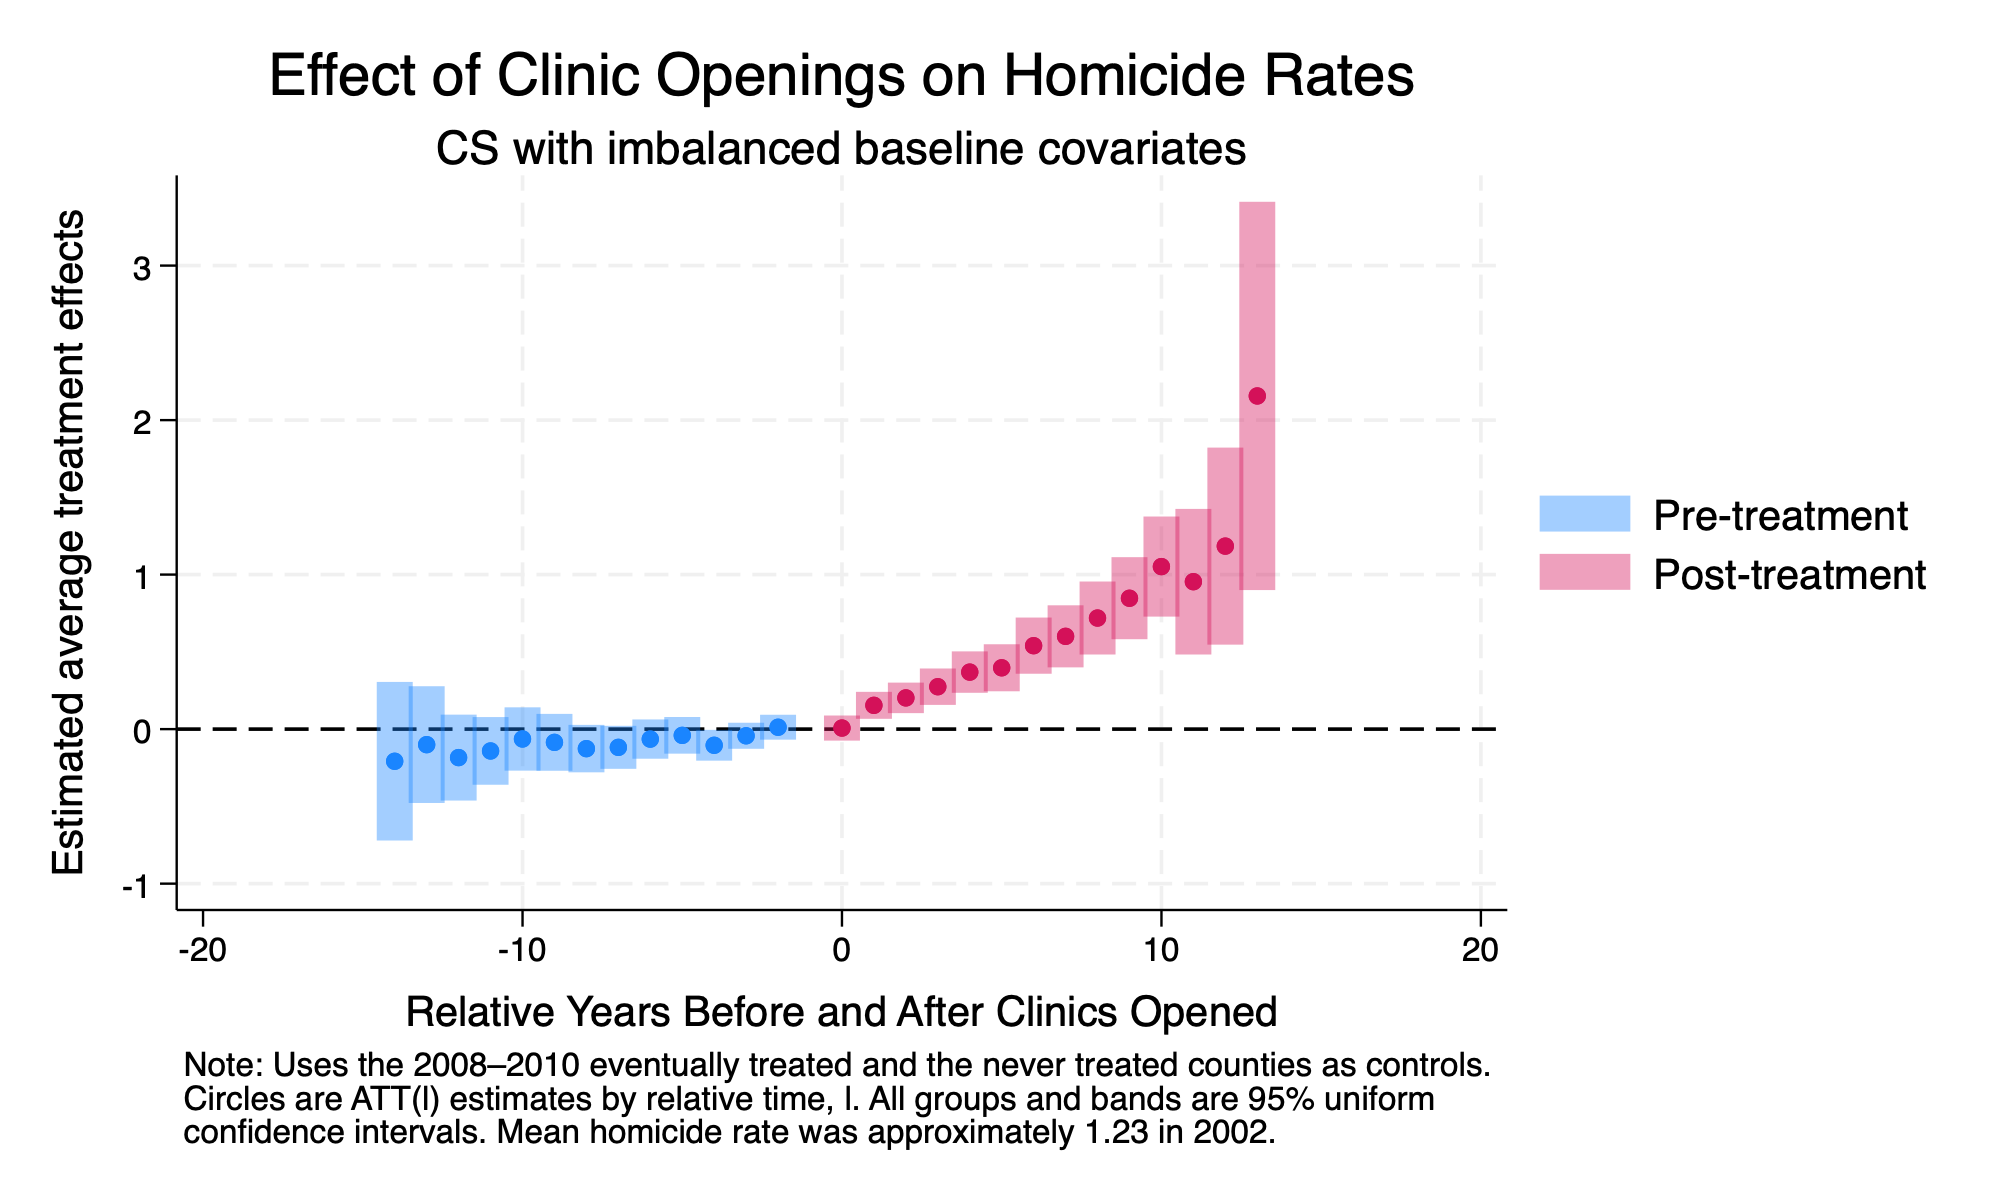
\includegraphics[height=0.72\textheight]{figures/brazil_cs_long2.png}
\end{center}
\begin{center}
\footnotesize\color{warmgray}\itshape
Years relative to CAPS opening. \;Bars are 95\% uniform confidence intervals. \;Pre-trend points near zero pass the falsification test.
\end{center}
\end{frame}

% =============================================================================
% STEP 9 — HonestDID sensitivity
% =============================================================================

\begin{frame}{Step 9: Sensitivity --- when pre-trends are imperfect}
\vspace{0.4cm}

Pre-trends rarely look \textit{exactly} flat. \;The question is then: \;how large would the parallel-trends violation have to be for our conclusion to flip?

\vspace{0.4cm}

\textbf{Rambachan \& Roth (2023),} \;\textit{``A More Credible Approach to Parallel Trends,''} \;\textit{Review of Economic Studies}, 90(5): 2555--2591.

\vspace{0.4cm}

\textbf{The idea.} \;Treat the magnitude of post-treatment parallel-trends violation as bounded by some multiple $M$ of the largest pre-period violation. \;For each $M$, compute the \textit{robust} confidence interval for the post-treatment effect. \;Then plot the CI as $M$ grows.

\vspace{0.4em}
\highlight{The estimator is no longer point-identified --- it's a set.} \;Honest about what the data can and cannot rule out.
\end{frame}

\begin{frame}[fragile]{Step 9 (cont.): the code}
\vspace{0.15cm}

The Stata implementation is the \texttt{honestdid} package (Rambachan, Roth, Wing). \;Two steps:

\begin{lstlisting}[language=Stata]
* 1. Estimate the CS event study with long2 / universal baseline
csdid2 homicide_rate $controls, gvar(g) ivar(cod) ///
    time(ano) long2 method(drimp) notyet
estat event, window(-4 5)

* 2. Run the sensitivity analysis on the post-period average
matrix l_vec = J(1, 1, 1)        // weight on Post_avg
honestdid, pre(3/5) post(2/2) ///
    mvec(0(0.25)2) delta(rm)  ///
    l_vec(l_vec) b(e(b)) vcov(e(V))
\end{lstlisting}

\vspace{0.1em}
\begin{itemize}\scriptsize\setlength\itemsep{0pt}
  \item \texttt{mvec(0(0.25)2)}: sweep $M$ from 0 to 2 in steps of 0.25.
  \item \texttt{delta(rm)}: relative-magnitudes restriction (the standard choice).
\end{itemize}
\end{frame}

\begin{frame}{Reading the HonestDID plot}
\vspace{0.25cm}

The output is a forest of confidence intervals, one for each $M$.

\vspace{0.3cm}
\begin{itemize}\small\setlength\itemsep{1pt}
  \item $M = 0$: the original CS estimate.
  \item $M = 0.5$: PT violation half as large as worst pre-period.
  \item $M = 1$: as large as worst pre-period.
  \item $M = 2$: twice as large.
\end{itemize}

\vspace{0.25cm}
\highlight{Breakdown point:} \;the $M$ at which the CI just touches zero. \;Surviving $M \geq 1$ means robust to anything seen in the pre-period.
\end{frame}

\begin{frame}{The HonestDID plot for CAPS}
\begin{center}
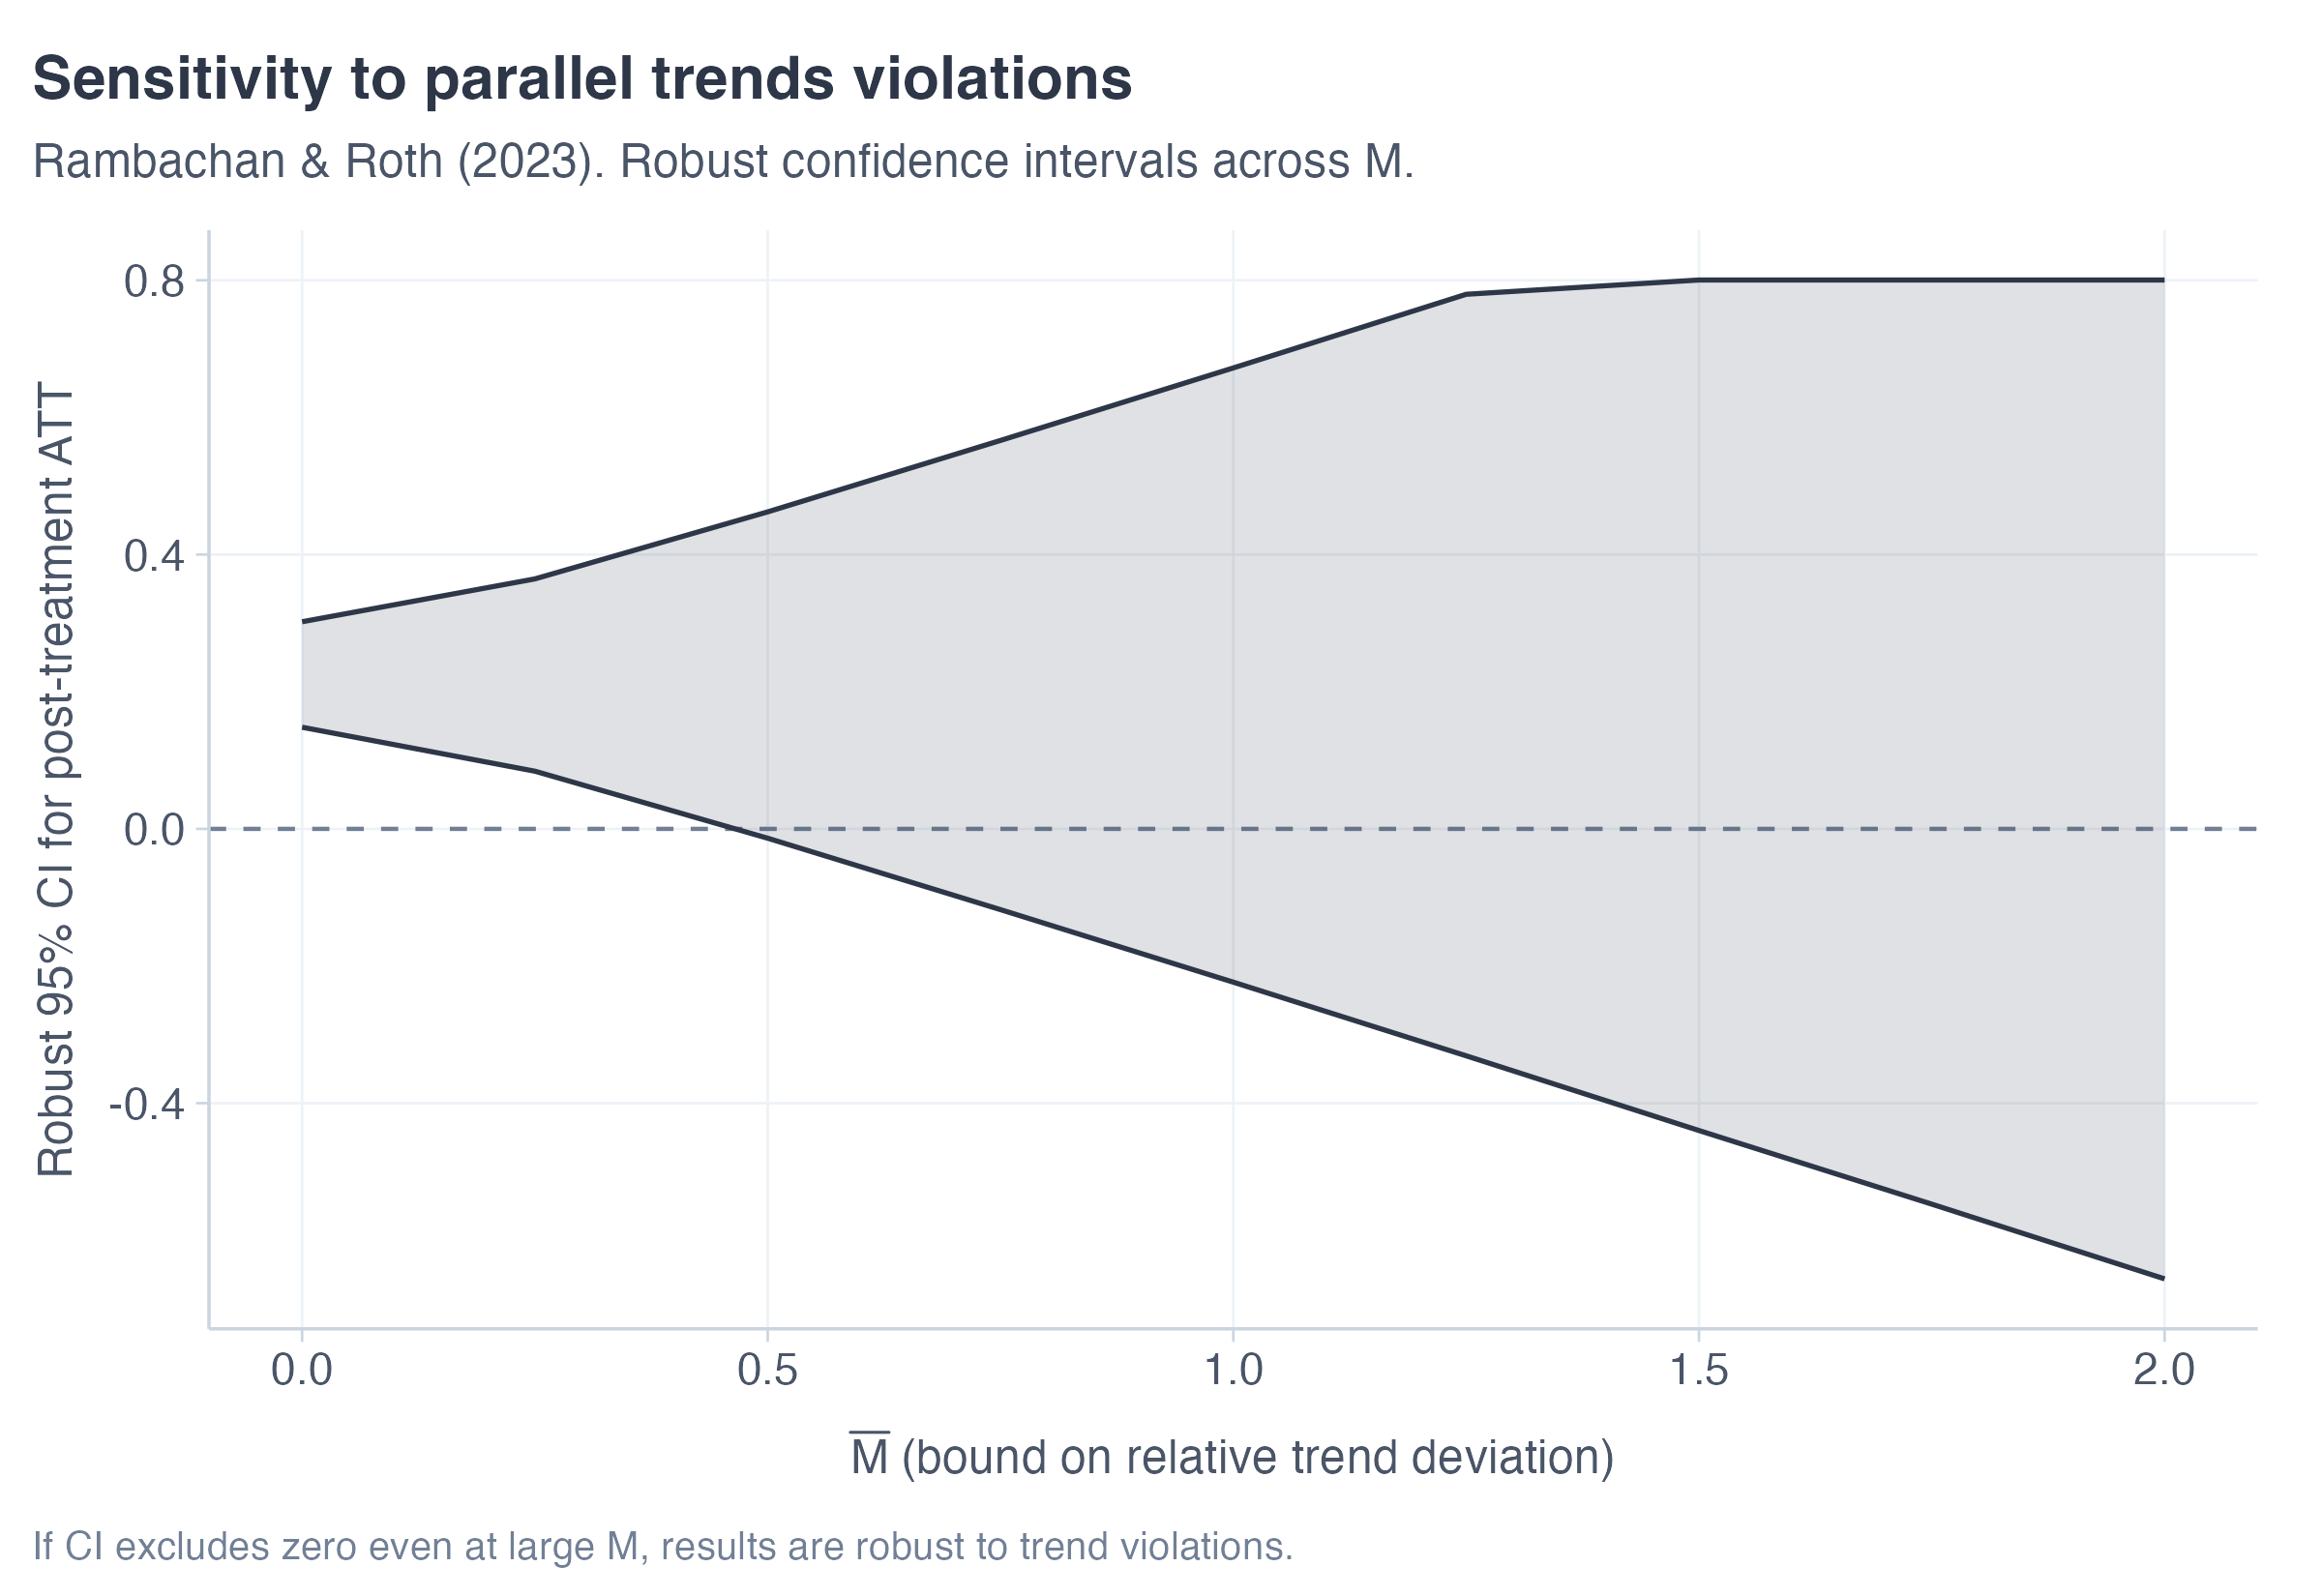
\includegraphics[height=0.72\textheight]{figures/brazil_honestdid.png}
\end{center}
\begin{center}
\footnotesize\color{warmgray}\itshape
Each bar is a 95\% robust CI for the post-treatment ATT at a value of $M$. \;Black diamond at $M=0$ is the original CS estimate.
\end{center}
\end{frame}

% =============================================================================
% CLOSING — Imbens, the 1970s crisis, knowing your data, tomorrow
% =============================================================================

\begin{frame}{A counterpoint: ``Don't Do DiD''}
\vspace{0.5cm}

\textbf{Guido Imbens} (Stanford, Nobel 2021) recently gave a talk titled \textit{``Don't Do Difference-in-Differences''} --- DDDiD.

\vspace{0.5cm}

\textbf{His argument.} \;Conditional parallel trends is a strong, untestable assumption. \;If you don't believe it, an estimator that requires it is the wrong tool. \;He recommends other panel methods --- chief among them \textbf{synthetic control} and \textbf{synthetic DiD}.

\vspace{0.6cm}

\meta{Imbens, \texttt{youtube.com/watch?v=GG627T4GbqU}}
\end{frame}

\begin{frame}{Why he might be right --- and the 1970s caution}
\vspace{0.4cm}

\textbf{The empirical crisis of the 1970s} was not a failure of econometrics. \;The math of 2SLS, regression, and instrumental variables is fine. \;Smart people could prove these results standing on their heads.

\vspace{0.5cm}

\textbf{What failed was the marriage of method to data.} \;Orley Ashenfelter and Janet Currie recall a time when researchers wouldn't even \textit{disclose what their instrument was}. \;Identification was assumed, not defended.

\vspace{0.5cm}

\highlight{The more complex the estimator, the higher the returns to knowing your data.} \;And the higher the cost of being wrong about its assumptions.
\end{frame}

\begin{frame}{But beware absolutes}
\vspace{0.5cm}

Many people will tell you that \textbf{including covariates in a DiD is always suspect.} \;Or that \textbf{you should never use TWFE under staggered adoption.} \;Or that \textbf{conditional parallel trends is too strong to defend.}

\vspace{0.5cm}

\textbf{Counter-example.} \;In the LaLonde--Dehejia--Wahba data, we just saw that conditional-on-$X$ DiD with the right covariates \textit{does} recover an estimate close to the RCT benchmark. \;Proof by contradiction.

\vspace{0.5cm}

\highlight{Don't throw rocks in glass houses.} \;The smart move is to know your data well enough to know when conditional PT might hold, when it might not, and to argue the case in both directions.
\end{frame}

\begin{frame}{Tomorrow: when you don't believe conditional PT}
\vspace{0.6cm}

If you have reason to doubt conditional parallel trends --- and you can't shore it up with covariates, sensitivity analysis, or design --- then you should be looking at a \textit{different} class of estimator.

\vspace{0.6cm}

\textbf{Tomorrow we cover:}
\begin{itemize}\setlength\itemsep{6pt}
  \item \textbf{Synthetic control} \;(Abadie, Diamond \& Hainmueller).
  \item \textbf{Synthetic DiD} \;(Arkhangelsky, Athey, Hirshberg, Imbens \& Wager).
\end{itemize}

\vspace{0.7cm}
\highlight{These trade one set of assumptions for another --- and that trade is the conversation worth having.}
\end{frame}

\end{document}
